\section{Zielsetzung}
\label{sec:zielsetzung}
Das im folgenden behandelte Experiment beschäftigt sich mit der Absorbtion und Emission von Röntgenstrahlung. Dabei wird zunächst die Bragg-Bedingung 
überprüft. Anschließend wird das Emissionsspektrum von Kupfer, sowie die Absorptionsspektren verschiedener Elemente wie Brom und Rubidium untersucht.
\section{Theorie}
\label{sec:theorie}
Die im Experiment verwendete Röntgenstrahlung wird durch eine Röntgenröhre erzeugt. In dieser werden in einer evakuirten Röhre freie Elektronen an einer Glühkathode erzeugt und anschließend zu einer Anode hin beschleunigt. Beim Auftreffen der Elektronen auf das Anodenmaterial wird von diesem Röntgenstrahlung emitiert.
\subsection{Röntgenemission}
\begin{figure}[h]
    \centering
    \includegraphics{Röntgenemission}
    \caption{Röntgenemission}
\end{figure}
Das Spektrum der emitierten Röntgenstrahlung ist stark vom verwendeten Anodenmaterial (in diesem Fall Kupfer) abhängig und wird in zwei verschiedene Unterkategorien von Spektren unterteilt. Diese Spektren, zum einen das kontinuirliche, zum anderen das charakteristische, unterscheiden sich grundlegend in der Form der Entstehung der jeweiligen Strahlung, die vom zugehörigen Spektrum beschrieben wird. \\
Das kontinuirliche Emissionsspektrum beschreibt die sogenannte Bremsstrahlung. Diese entsteht, wenn ein Elektron sich einem Nukleon nähert und in dessen Coulombfeld abgelenkt bzw. abgebremst wird, wobei das Elektron einen Teil seiner (kinetischen) Energie abgibt. Bei diesem Vorgang wird ein Röntgenquant emittiert, dessen Energie der Energiedifferenz des Elektrons entspricht.
\begin{equation}
E_{ph}=hf=E_{0.kin}-E_{kin}
\end{equation}
Da das Elektron Situationsabhängig beliebig stark gebremst, also einen beliebigen Anteil seiner kinetischen Energie abgeben kann, ist dieser Teil des Spektrums kontinuirlich. Für den Grenzfall, bei dem das Elektron seine gesamte kinetische Energie abgibt, ergibt sich die maximale Energie, und somit die minimale Wellenlänge des Spektrums. Für diesen Fall lässt sich aus der Beziehung $\frac{hc}{\lambda_{min}}=Ue$ die minimale Wellenlänge
\begin{equation}
\lambda_{min}=\frac{hc}{Ue}
\end{equation}
mit der Beschleunigungsspannung U und dem Planckschen Wirkungsquantum h bestimmen. \\
Das sogenannte characteristische Spektrum entsteht, wenn das einfallende Elektron ein Atom derart ionisiert, dass eine Leerstelle in einer der inneren Schalen des Atoms entsteht. Diese Leerstelle wird von einem Elektron aus einer der äußeren Schalen eingenommen was zur Emission eines Röntgenquants führt, dessen Energie der Differenz der Bindungsenergien beider Schalen entspricht ($E=E_m-E_n$). \\
Da die einzelnen Energieniveaus und daraus folgend die zugehörige Röntgenstrahlung spezifisch für das verwendete Anodenmaterial ist, tritt diese Form der Röntgenstrahlung nur mit bestimmten diskreten Energiewerten auf, die sich im Spektrum durch scharfe Linien zeigt. Dieses Spektrum ist also nicht kontinuirlich und charakteristisch für das Anodenmaterial der verwendeten Röntgenröhre. \\
Die betreffenden Linien werden in der Form $K_\alpha$, $K_\beta$, $L_\alpha$ usw. bezeichnet. Wobei der Buchstabe K/L... die innere Schale bezeichnet, auf die das Elektron übergeht, während der griechische Buchstabe im Index auf die Herkunft des Elektrons, also die Schale aus der das Elektron übergesprungen ist schließen lässt. \\
Die Berechnung der Bindungsenergie eines Elektrons auf der n-ten Schale ist essentiell um die theoretische Energie der charakteristischen Röntgenstrahlung bestimmen zu können. Diese Bindungsenergie kann mithilfe der Formel
\begin{equation}
E_n=-R_{\infty}z_{eff}^2\frac{1}{n^2}
\end{equation}
mit der Rydbergenergie $R_{\infty}=13,6 eV$ berechnet werden. Die Abschirmung der äußeren Elektronen von der Kernladung, die in einem Atom mit mehreren besetzten Elektronenschalen auftritt, wird hier in der effektiven Kernladungszahl $z_{eff}=Z-\sigma$ durch die Abschirmkonstante $\sigma$ berücksichtigt. Diese variirt von Elektron zu Elektron und kann empirisch bestimmt werden.
Da die Hüllenelektronen sich durch Bahndrehimpuls und Elektronenspin unterscheiden, ist auch die Bindungsenergie nicht bei allen Elektronen identisch. Dadurch ist das charakteristische Spektrum meist in mehrere Linien gegliedert. Dieses Phänomen wird Feinstruktur genannt und muss in einigen Berechnungen berücksichtigt werden.
\subsection{Röntgenabsorption}
\begin{figure}[h]
    \centering
    \includegraphics{Röntgenabsorption}
    \caption{Röntgenabsorption}
\end{figure}
Die Absorption von Röntgenstrahlung geschieht vornehmlich durch den Photoeffekt, sowie durch die Verringerung der Photonenenergie durch den Compton-Effekt. Dabei verringert sich das Maß der Absorption mit steigender Energie der einfallenden Röntgenstrahlung, bis diese einen Wert etwas größer der Bindungsenergie einer der inneren Schalen erreicht. Sobald dieser Wert erreicht wird, kann das Photon das Atom ionisieren und der Absorptionskoeffizient steigt infolge dessen sprunghaft an.
Diese Sprünge im Absorptionsspektrum werden als K-/M-/L-Kante, je nach Schale des herausgeschlagenen Elektrons, bezeichnet. Der Energiewert der betreffenden Röntgenstrahlung beträgt $hf=E_m-E_{\infty}$ und kann näherungsweise als Bindungsenergie der Schale angenommen werden. 
Wenn der Wert der K-Kante $E_K$ bekannt ist, kann die Abschirmkonstante für Elektronen der K-Schale durch die Formel
\begin{equation}
\sigma_K=Z-\sqrt{\frac{E_K}{R_{\infty}}-\frac{\alpha^2Z^4}{4}}
\end{equation}
berechnet werden. Hier bezeichnet $\alpha$ die Sommerfeldsche Feinstrukturkonstante. 
\subsection{Bragg-Reflexion}
\begin{figure}[h]
    \centering
    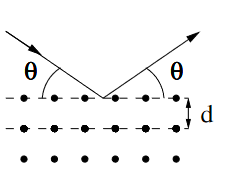
\includegraphics{Bragg-Reflexion}
    \caption{Bragg-Reflexion}
\end{figure}
Die Wellenlänge, und im Zuge dessen die Energie, von Röntgenstrahlung kann empirisch mithilfe der Bragg-Reflexion bestimmt werden. Diese tritt auf, wenn einfallende Röntgenstrahlung an einem Kristallgitter gebeugt wird. Durch die Gitterstruktur tritt ein Weglängenunterschied zwischen den Strahlen auf. Unter dem sogenannten Glanzwinkel $\Theta$ beträgt dieser Gangunterschied ein (ganzzahliges) Vielfaches der Wellenlänge, und es lässt sich konstruktive Interferenz beobachten. Aus dieser Bedingung lässt sich die Gleichung
\begin{equation}
2dsin(\Theta)=n\lambda
\end{equation}
für die Wellenlänge herleiten. n beschreibt hier die Ordnung der Reflexion und d die Gitterkonstante, die für den in diesem Versuch verwendeten LiF-Kristall $d=201,4 pm$ beträgt.
